\documentclass{beamer}
\setbeamertemplate{footline}[frame number]
%\usepackage{beamerthemeBerkeley}
\usetheme{Montpellier}
%\usetheme{Warsaw}
%\usetheme{Boadilla}
\usepackage[english]{babel}
\usepackage{graphicx}
%\usepackage{ams}
%\usepackage{blue}
\usepackage{amsmath} 


\title{Lecture 1: Case Control Association Testing \& Association Testing with Quantitative Traits}

\author{Instructors: Joelle Mbatchou and Loic Yengo} 


\date{}


\begin{document}



\begin{frame}
\titlepage
\vspace{-2cm}
\begin{center}

{ \Large Summer Institute in Statistical Genetics 2022\\}


\end{center}
\end{frame}

%\maketitle


\begin{frame}
\frametitle{\bf Introduction}
\begin{itemize}
\item Association mapping is now routinely being used to identify loci
that are involved with complex traits.
\item Technological advances have made it feasible to perform association studies
on a genome-wide basis with millions of markers in a single study.
\item  We consider testing a genetic marker for association with a disease (e.g. 1/0, affected/unaffected, dead/alive) or a quantitative trait (e.g. height, BMI) in \textbf{a sample of unrelated subjects}.
\item Vast amounts of literature on these topics!  
\end{itemize}
\end{frame}


%% CC association testing
\begin{frame}
\frametitle{\bf Case-Control Association Testing}
\begin{itemize}

\item Allelic Association Tests
  \begin{itemize}
\item Allele is treated as the sampling unit
\item Typically make an assumption of Hardy-Weinberg equilibrium (HWE) - alleles within an individual are conditionally independent given the disease status
\item e.g. Pearson's $\chi^2$ 
\end{itemize}
\item Genotypic Association Tests
\begin{itemize}
\item Individual is the sampling unit
\item Does not assume HWE
\item e.g. Logistic regression
\end{itemize}
\end{itemize}
\end{frame}

\section{Allelic Association Tests}

\begin{frame}
\frametitle{\bf Pearson's $\chi^2$ Test for Allelic Association}
\begin{itemize}
%\item The classical Pearson's $\chi^2$ test is often used for allelic association testing.
\item This test looks for deviations from independence between the trait and allele.
\item Consider a single marker with 2 allelic types (e.g., a SNP) labeled "C"' and "T"'.
\item Let $N_{ca}$ be the number of cases and $N_{co}$ be the number of controls on which we have genotype data.
\end{itemize}
\end{frame}

\begin{frame}
\frametitle{\bf Pearson's $\chi^2$ Test for Allelic Association}
\begin{itemize}
\item Below is a 2$\times$2 contingency table for trait and allelic type   \\

    \begin{center}
      \begin{tabular}{|c|cc|c|}
        \hline
         & Cases & Controls & Total\\
 \hline
  Allele C& $n^{ca}_{C}$ & $n^{co}_{C}$ &$N_C$   \\
  Allele T& $n^{ca}_{T}$ &$ n^{co}_{T}$& $N_T$\\
 \hline
 Total& $2N_{ca}$ & $2N_{co}$ & $2N$ \\
 \hline
      \end{tabular}
    \end{center}


\item $n^{ca}_C$ is the number of C alleles in the cases and $n^{ca}_C=$ 2 $\times$ the number of homozygous CC cases  $+$ the number of heterozygous CT cases
\item Hypotheses
\begin{itemize}

  \item $H_0$: there is \textit{no association} between the row variable and column variable
  \item $H_a$: there \textit{is} an association between the two variables
  \end{itemize}
   \end{itemize}
\end{frame}


\begin{frame}
\frametitle{\bf Pearson's $\chi^2$ Test for Allelic Association}
\begin{itemize}
\item Can use Pearson's $\chi^2$ test for independence. The statistic is:

  \[ X^2 = \sum_{\mbox{all cells}} \frac{\left(\mbox{Observed cell} - \mbox{
        Expected cell}\right)^2}{\mbox{Expected cell }} \]
\item What is the the expected cell number under $H_0$? For each cell, we have
  \[ \mbox{Expected Cell Count} = \frac{\mbox{row total } \times
    \mbox{ col total}}{\mbox{total count}} \]
\item Under $H_0$, the $X^2$ test statistic has an approximate $\chi^2$
  distribution with $(r-1)(c-1)=(2-1)(2-1)=1$ degree of freedom
\end{itemize}
\end{frame}


\begin{frame}
\frametitle{\bf LHON Example: Pearson's $\chi^2$ Test }
\begin{itemize}
\item From Phasukijwattana et al. (2010), Leber Hereditary Optic Neuropathy (LHON) disease and genotypes for marker rs6767450:\\

    \begin{center}
      \begin{tabular}{|c|ccc|}
        \hline
         & CC & CT & TT\\
 \hline
  Cases & 6 & 8 &75 \\
  Controls& 10&66& 163\\
 \hline
      \end{tabular}
    \end{center}


\item Corresponding $2 \times 2$ contingency table with allelic type instead of genotype
    \begin{center}
      \begin{tabular}{|c|cc|}
        \hline
         & Allele C  &  Allele T\\
 \hline
  Cases & 20 & 158  \\
  Controls &86& 39 \\
 \hline
      \end{tabular}
    \end{center}
\item Should we reject the hypothesis that allelic type is independent of disease status?
\end{itemize}
\end{frame}


\begin{frame}
\frametitle{\bf LHON Example: Pearson's $\chi^2$  Test }
  \begin{center}
      \begin{tabular}{|c|cc|c|}
        \hline
         & Allele C  &  Allele T& Total\\
\hline
Cases & 20 & 158 & 178   \\
Controls &86& 392 &478 \\
\hline
Total& 106&550& 656 \\
 \hline
      \end{tabular}
    \end{center}
\begin{itemize}
\item Intuition for the test: Suppose $H_0$ is true, so allelic type and case-control status are independent, then what counts would we expect?
\begin{itemize}
\item the expected number of case alleles that are of type C is:
\begin{align*}
n^{ca}_T &= \{\#cases\} \times P(\mbox{Allelic type is C  \(|\)  Allele is from a Case}) \\
&=  \{\#cases\}  \times P(\mbox{Allelic type is C}) \quad \textbf{(independence)}\\
&=178\times \left(\frac{106}{656}\right)=28.7622
\end{align*}
\end{itemize}
\end{itemize}
\end{frame}


\begin{frame}
\frametitle{\bf LHON Example: Pearson's $\chi^2$ Test }
 \begin{itemize}
\item Fill in the remaining cells for the expected counts
  \begin{center}
      \begin{tabular}{|c|cc|c|}
        \hline
         & Allele C  &  Allele T& Total\\
\hline
Cases & 28.7622 & . & 178   \\
Controls &.& . &478 \\
\hline
Total& 106&550& 656 \\
 \hline
      \end{tabular}
    \end{center}
 \end{itemize}
\end{frame}




\begin{frame}
\frametitle{\bf LHON Example: Pearson's $\chi^2$ Test }
 \begin{itemize}
\item<1-> Fill in the remaining cells for the expected counts
  \begin{center}
      \begin{tabular}{|c|cc|c|}
        \hline
         & Allele C  &  Allele T& Total\\
\hline
Cases & 28.7622 & 149.2378 & 178   \\
Controls &77.2378& 400.7622  &478 \\
\hline
Total& 106&550& 656 \\
\hline
      \end{tabular}
    \end{center}
\item<2-> Calculate the $X^2$ statistic
 \[X^2=\frac{(20-28.7622)^2}{28.7622}+\cdots+\frac{(392-400.7622 )^2}{400.7622 }=4.369\]
\item<3-> What is the $p$-value?

\[ P(\chi ^2_{1} \ge 4.369)=.037 \]
\end{itemize}
\end{frame}

\section{Genotypic Association Tests}



\begin{frame}
\frametitle{\bf Odds Ratios (ORs) for Genotypes}
\begin{itemize}
\item What are \textbf{odds}? An expression of \textbf{relative probabilities}...
\end{itemize}
\centering	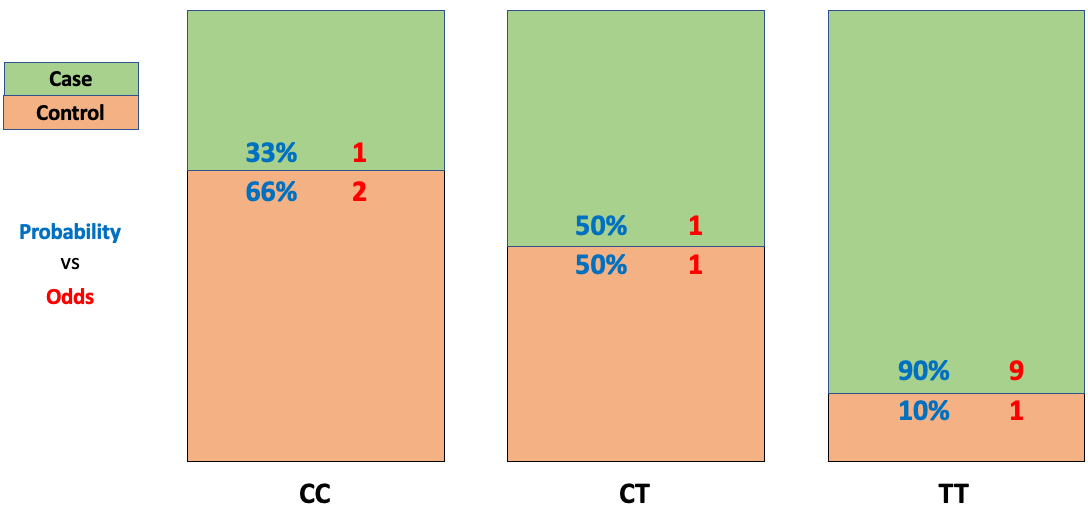
\includegraphics[scale=.35]{Figures/odds_plot1.png}
\vspace{-1em}
\begin{itemize}
	\item Odds of disease in an individual with the CC genotype = 50\%
\end{itemize}
\end{frame}


\begin{frame}
	\frametitle{\bf Odds Ratios (ORs) for Genotypes }
	\centering	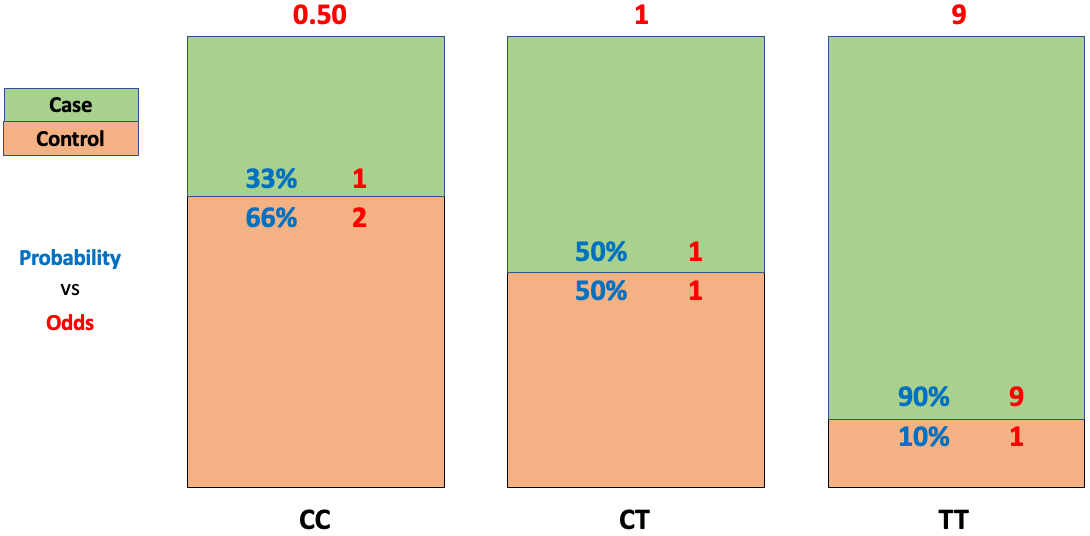
\includegraphics[scale=.2]{Figures/odds_plot2.png}
\begin{itemize}
\item Typically choose a reference genotype, e.g. CC
\[ OR_{TT} =\frac{\mbox{odds of disease with the TT genotype}}{\mbox{odds of disease with the CC genotype}} =\frac{9}{0.50} = 18 \]

\item $OR_{TT}=1$ implies no association with disease.  
\item $OR_{TT}>1$ or $OR_{TT}<1$ implies association with the disease.  
 \end{itemize}

\end{frame}


\begin{frame}
	\frametitle{\bf Genotypic Association Tests: Logistic regression }
\begin{itemize}
\item  Generally used to estimate odds ratios and get confidence intervals for genotypes.
\item Let $\pi_i$ be the probability that individual $i$ is has the disease and  let  $G_i$ be the genotype at the SNP:
\begin{align*}
\log\underbrace{\left(\frac{\pi_i}{1-\pi_i}\Big|G_i\right)}_{\text{odds of disease}} &=
\beta _0 + \beta _{CT}I\{G_i=CT\}+\beta_{TT}I\{G_i=TT\}
\end{align*}
% log(odds of disease for individual i|G_i) &=
 where $I\{G_i=CT\}$ is 1 if $G_i=CT$ and 0 otherwise, and similarly for $I\{G_i=TT\}$.
\end{itemize}
\end{frame}

\begin{frame}
\frametitle{\bf Genotypic Association Tests: Logistic regression }
\begin{itemize}

\item The coefficient estimates for $\hat{\beta}_{CT}$ and $\hat{\beta}_{TT}$ can be used to calculate odds ratios:
\begin{align*}
	OR_{CT} &=\frac{\mbox{odds of disease with the CT genotype}}{\mbox{odds of disease with the CC genotype}} \\
	& = \frac{exp(\hat{\beta} _0  + \hat{\beta}_{CT})}{exp(\hat{\beta}_0 )}
	= exp(\hat{\beta}_{CT})
\end{align*}
Similarly, $OR_{TT}=exp(\hat{\beta}_{TT}) $
\item 95\% CI for $OR_{CT}$ is
\[ exp(\hat{\beta}_{CT} \pm 1.96\times s.e.(\hat{\beta}_{CT})) \]
\end{itemize}
\end{frame}

\begin{frame}
\frametitle{\bf Odds Ratios for LHON Example }

\begin{itemize}
\item Leber Hereditary Optic Neuropathy (LHON) disease and genotypes for marker rs6767450:\\

    \begin{center}
      \begin{tabular}{|c|c|c|c|}
        \hline
         & CC & CT & TT\\
 \hline
  Cases & 6 & 8 &75 \\
  \hline
  Controls& 10&66& 163\\
 \hline
      \end{tabular}
    \end{center}

\item We will use the \texttt{R} to obtain odds ratios and confidence intervals for this data set 
\item We will contrast this test with an allelic test (Pearson's $\chi^2$ test).
%\item Exercises and some commands for analyzing the LHON data with  \texttt{R} can be found on the following webpage:\\
%\vspace{.5em}
%\url{https://joellembatchou.github.io/SISG2022_Association_Mapping/}
\end{itemize}



\end{frame}




\section{QTL mapping}

%% QTL mapping

\begin{frame}
	\frametitle{\bf Introduction to Quantitative Trait Mapping}
	\begin{itemize}
		\item Quantitative trait loci (QTL) mapping involves identifying genetic loci that influence the phenotypic variation of a quantitative trait.
		\item QTL mapping is commonly conducted with GWAS, often involving directly genotyped variants along with imputation through reference panels to result in millions of genetic variants
		\item	Some quantitative traits can be largely influenced by a single gene as well as by environmental factors (e.g. monogenic or Mendelian traits)
	\end{itemize}
\end{frame}

\begin{frame}
	\frametitle{\bf Introduction to Quantitative Trait Mapping}
	\begin{itemize}
		\item  Influences on a quantitative trait can also be due to a number of genes  (polygenicity)
		\item Many quantitative traits of interest are complex where phenotypic variation is due to a combination of both multiple genes and environmental factors
		\item Examples: Blood pressure, cholesterol levels, IQ, height, weight, etc.
	\end{itemize}
\end{frame}


\begin{frame}
	\frametitle{\bf Quantitative Genetic Model}
	\begin{itemize}
		\item The classical quantitative genetics model introduced by Ronald Fisher (1918) is $Y=G+E $, where $Y$ is the phenotypic value, $G$ is the genetic value, and $E$ is the environmental deviation.
		\item $G$ is the combination of all genetic loci that influence the phenotypic value  and $E$ consists of all non-genetic factors that influence the phenotype
		\item The mean environmental deviation $E$ is generally taken to be 0 so that the mean genotypic value is equal to the mean phenotypic value, i.e., $E(Y)=E(G)$
	\end{itemize}
\end{frame}

\begin{frame}
	\frametitle{\bf Components of Genetic Variance }
	\begin{itemize}
		\item Consider a single locus.  Fisher modeled the genotypic value $G$ with a linear regression model (least squares) where the genotypic value can be partitioned into an additive component ($A$) and deviations from additivity as a result of dominance ($D$), where 
		\vspace{-1em}
		\begin{align*}
		G &=A+ D ,\\
		\underbrace{Var(G)}_{\sigma^2_{G}}&= \underbrace{Var(A)}_{\sigma^2_{A}}+ \underbrace{Var(D)}_{\sigma^2_{D}} 
		\end{align*}
		\vspace{-0.5em}
		\item $\sigma^2_{A}$ is the \textbf{additive genetic variance}.  It is the genetic variance associated with the average additive effects of alleles
		\item  $\sigma^2_{D}$ is the \textbf{dominance genetic variance}. It is the genetic variance associated with the dominance effects.
		
		
	\end{itemize}
	
\end{frame}


\begin{frame}
	\frametitle{\bf Heritability}
	\begin{itemize}
		\item Remember that $Y=G+E = A+D+E$ 
		\item {\bf Narrow-sense heritability} (or simply heritability) is defined as
		\[ h^2 = \frac{    \sigma^2_{A} }    {  \sigma^2_{Y}   } \]
	\item   $h^2$ is the proportion of the total phenotypic variance that is due to additive effects. 
		\item Heritability can also be viewed as  the extent to which phenotypes are determined by the alleles transmitted from the parents.   
	\end{itemize}
\end{frame}


\begin{frame}
	\frametitle{\bf Heritability}
	\begin{itemize}
		\item The {\bf broad-sense heritability} is defined to be
		\[ H^2 = \frac{    \sigma^2_{G} }    {  \sigma^2_{Y}   } \]
		\item $H^2$  is the proportion of the total phenotypic variance that is due to all genetic effects (additive and dominance)
		\item Heritability can vary over time and with  the study population as it depends also on environmental effects
	\end{itemize}
\end{frame}



\begin{frame}
	\frametitle{\bf  QTL Mapping}
	\begin{itemize}
		\item For traits that are heritable, i.e., traits with a non-negligible genetic component that contributes to phenotypic variability, identifying (or mapping) QLT  that influence the trait is often of interest.
		\item Linear regression models are commonly used for QTL mapping

		\begin{itemize}
		\item They will often include a single genetic marker (e.g., a SNP) as predictor in the model, in addition to other relevant covariates (e.g. age, sex), with the quantitative phenotype as the response
	\end{itemize}

\end{itemize}
\end{frame}


\begin{frame}
	\frametitle{\bf Linear regression with SNPs}
	
	Many analyses fit the `additive model'
	\[
	y = \beta_0 + \beta\times\#\mbox{T alleles}
	\]
	
	\centerline{
		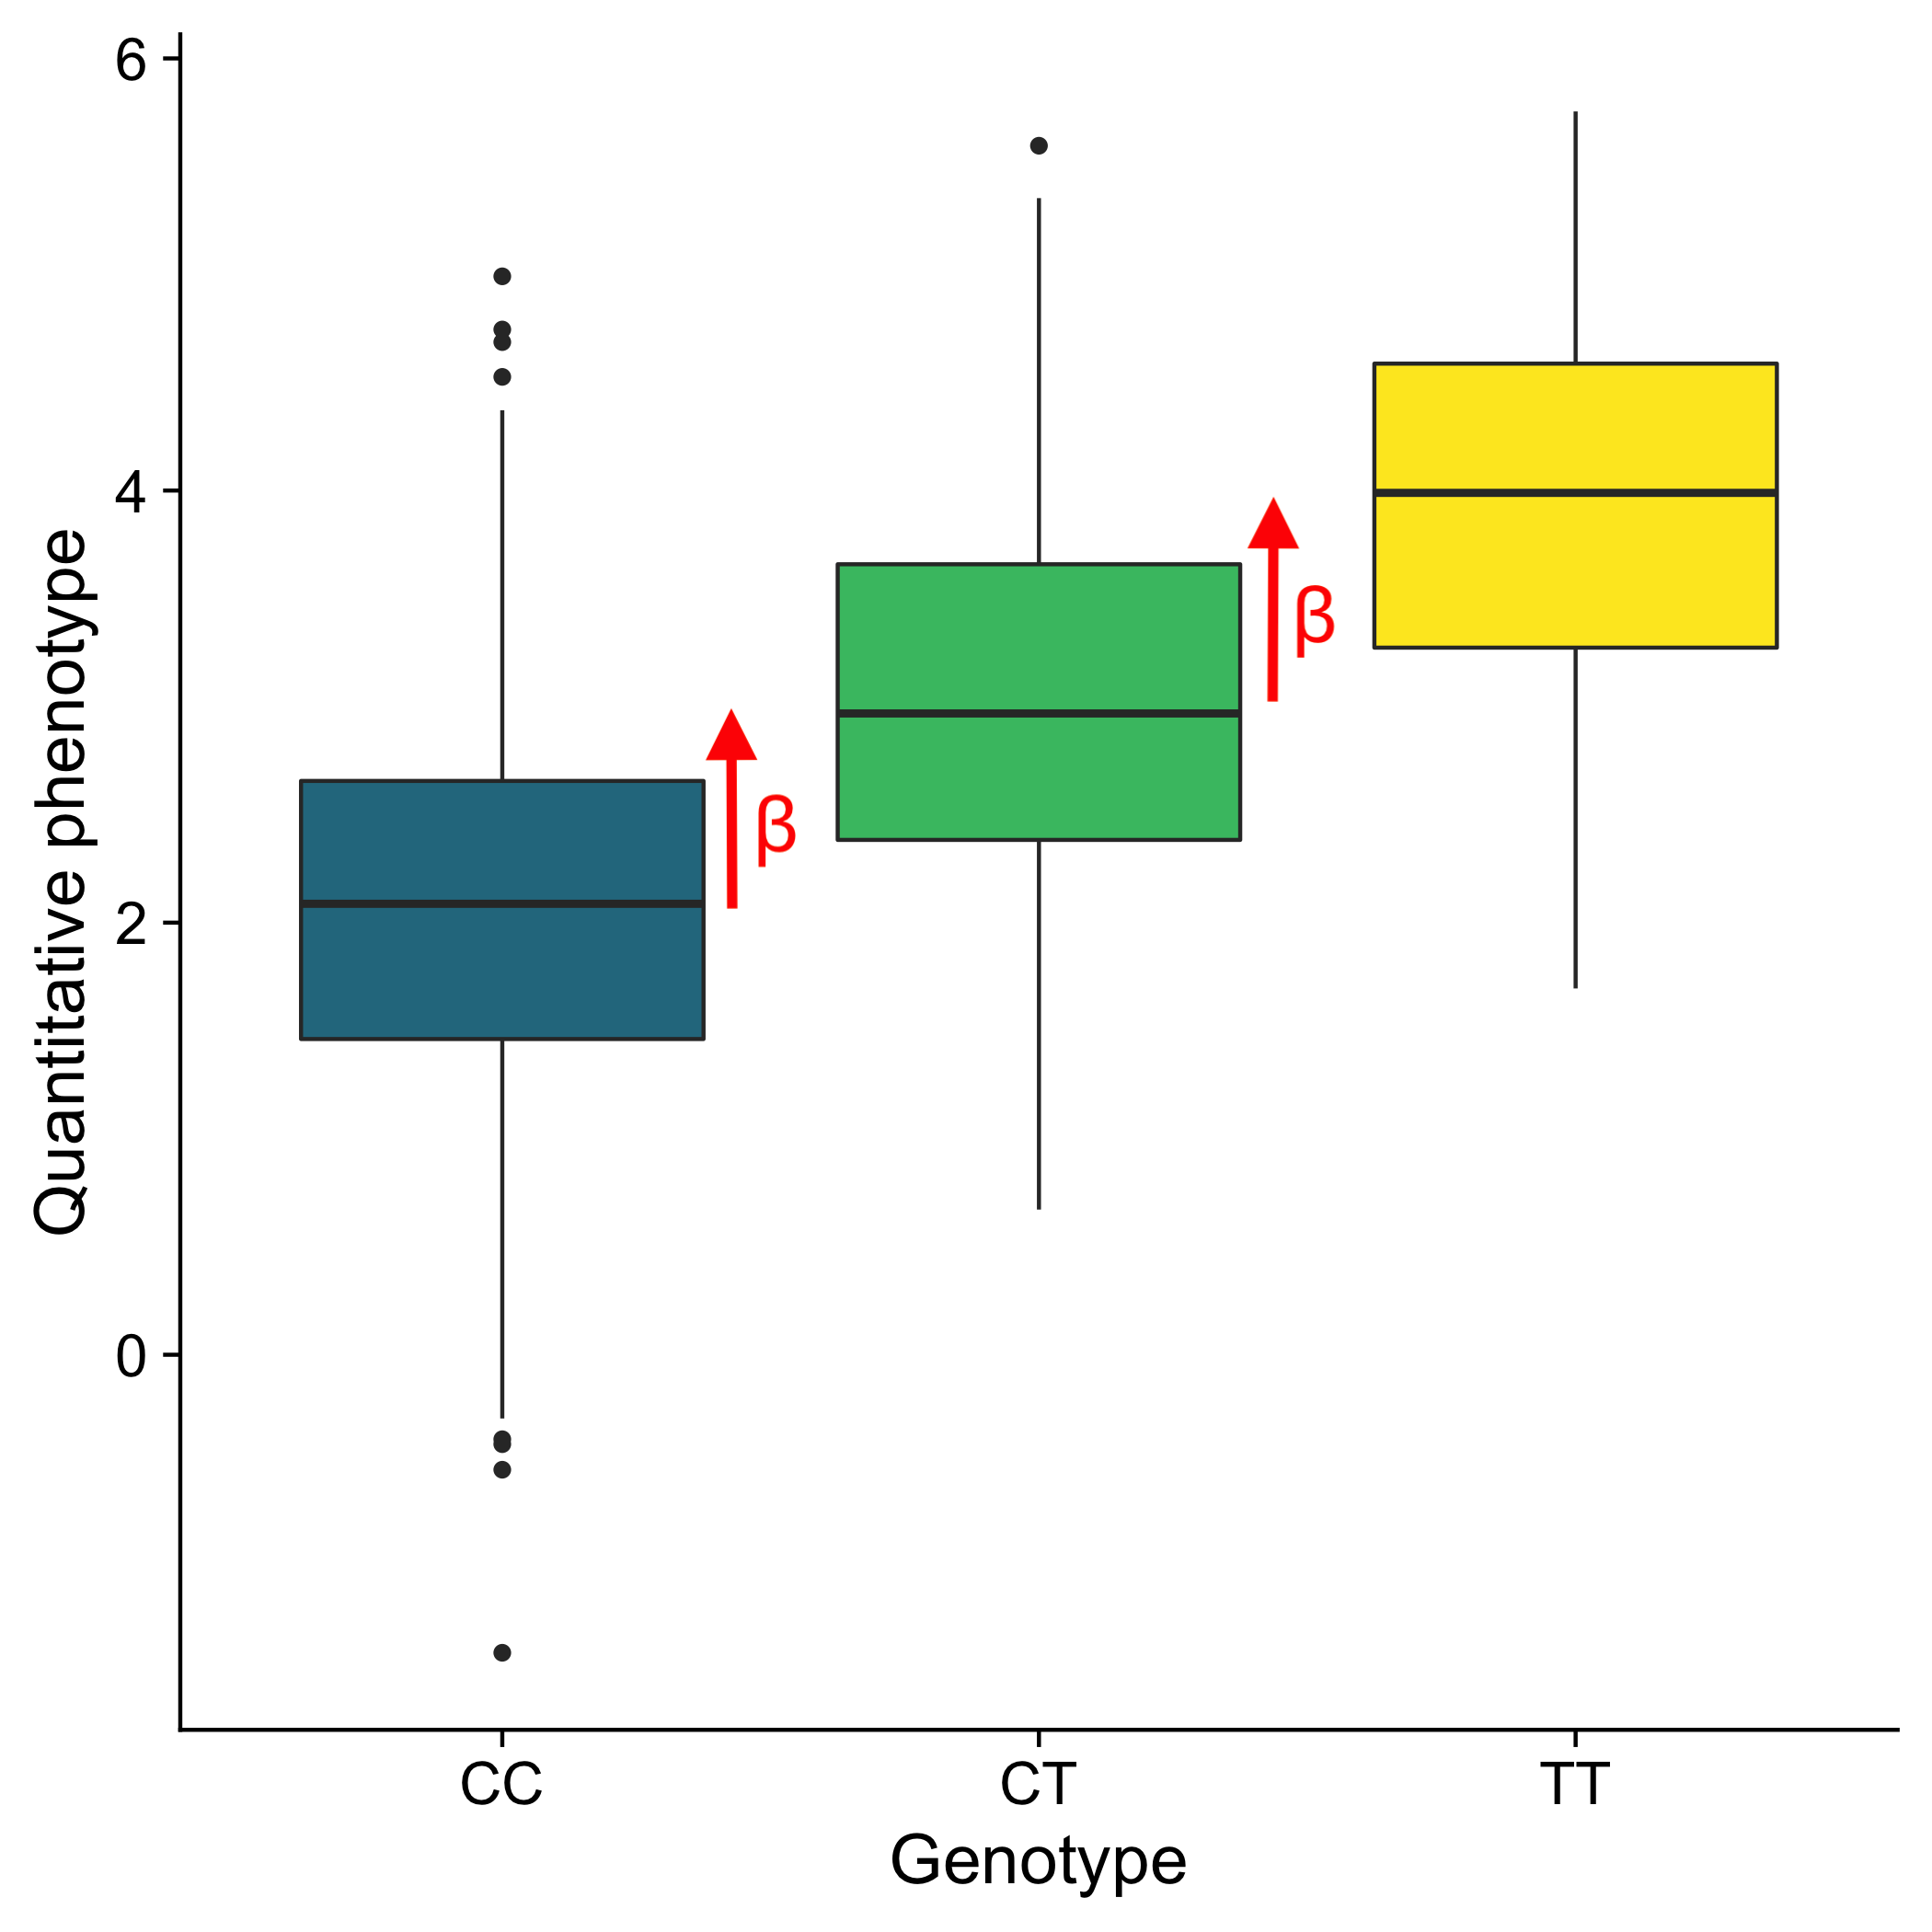
\includegraphics[scale=.08]{Figures/lm_add.png}
	}
	
\end{frame}

\begin{frame}
	\frametitle{\bf Linear regression, with SNPs}
	
	An alternative is the `dominant model';
	\[
	y = \beta_0 + \beta\times I\{G\neq CC\}
	\]
	
	\centerline{
		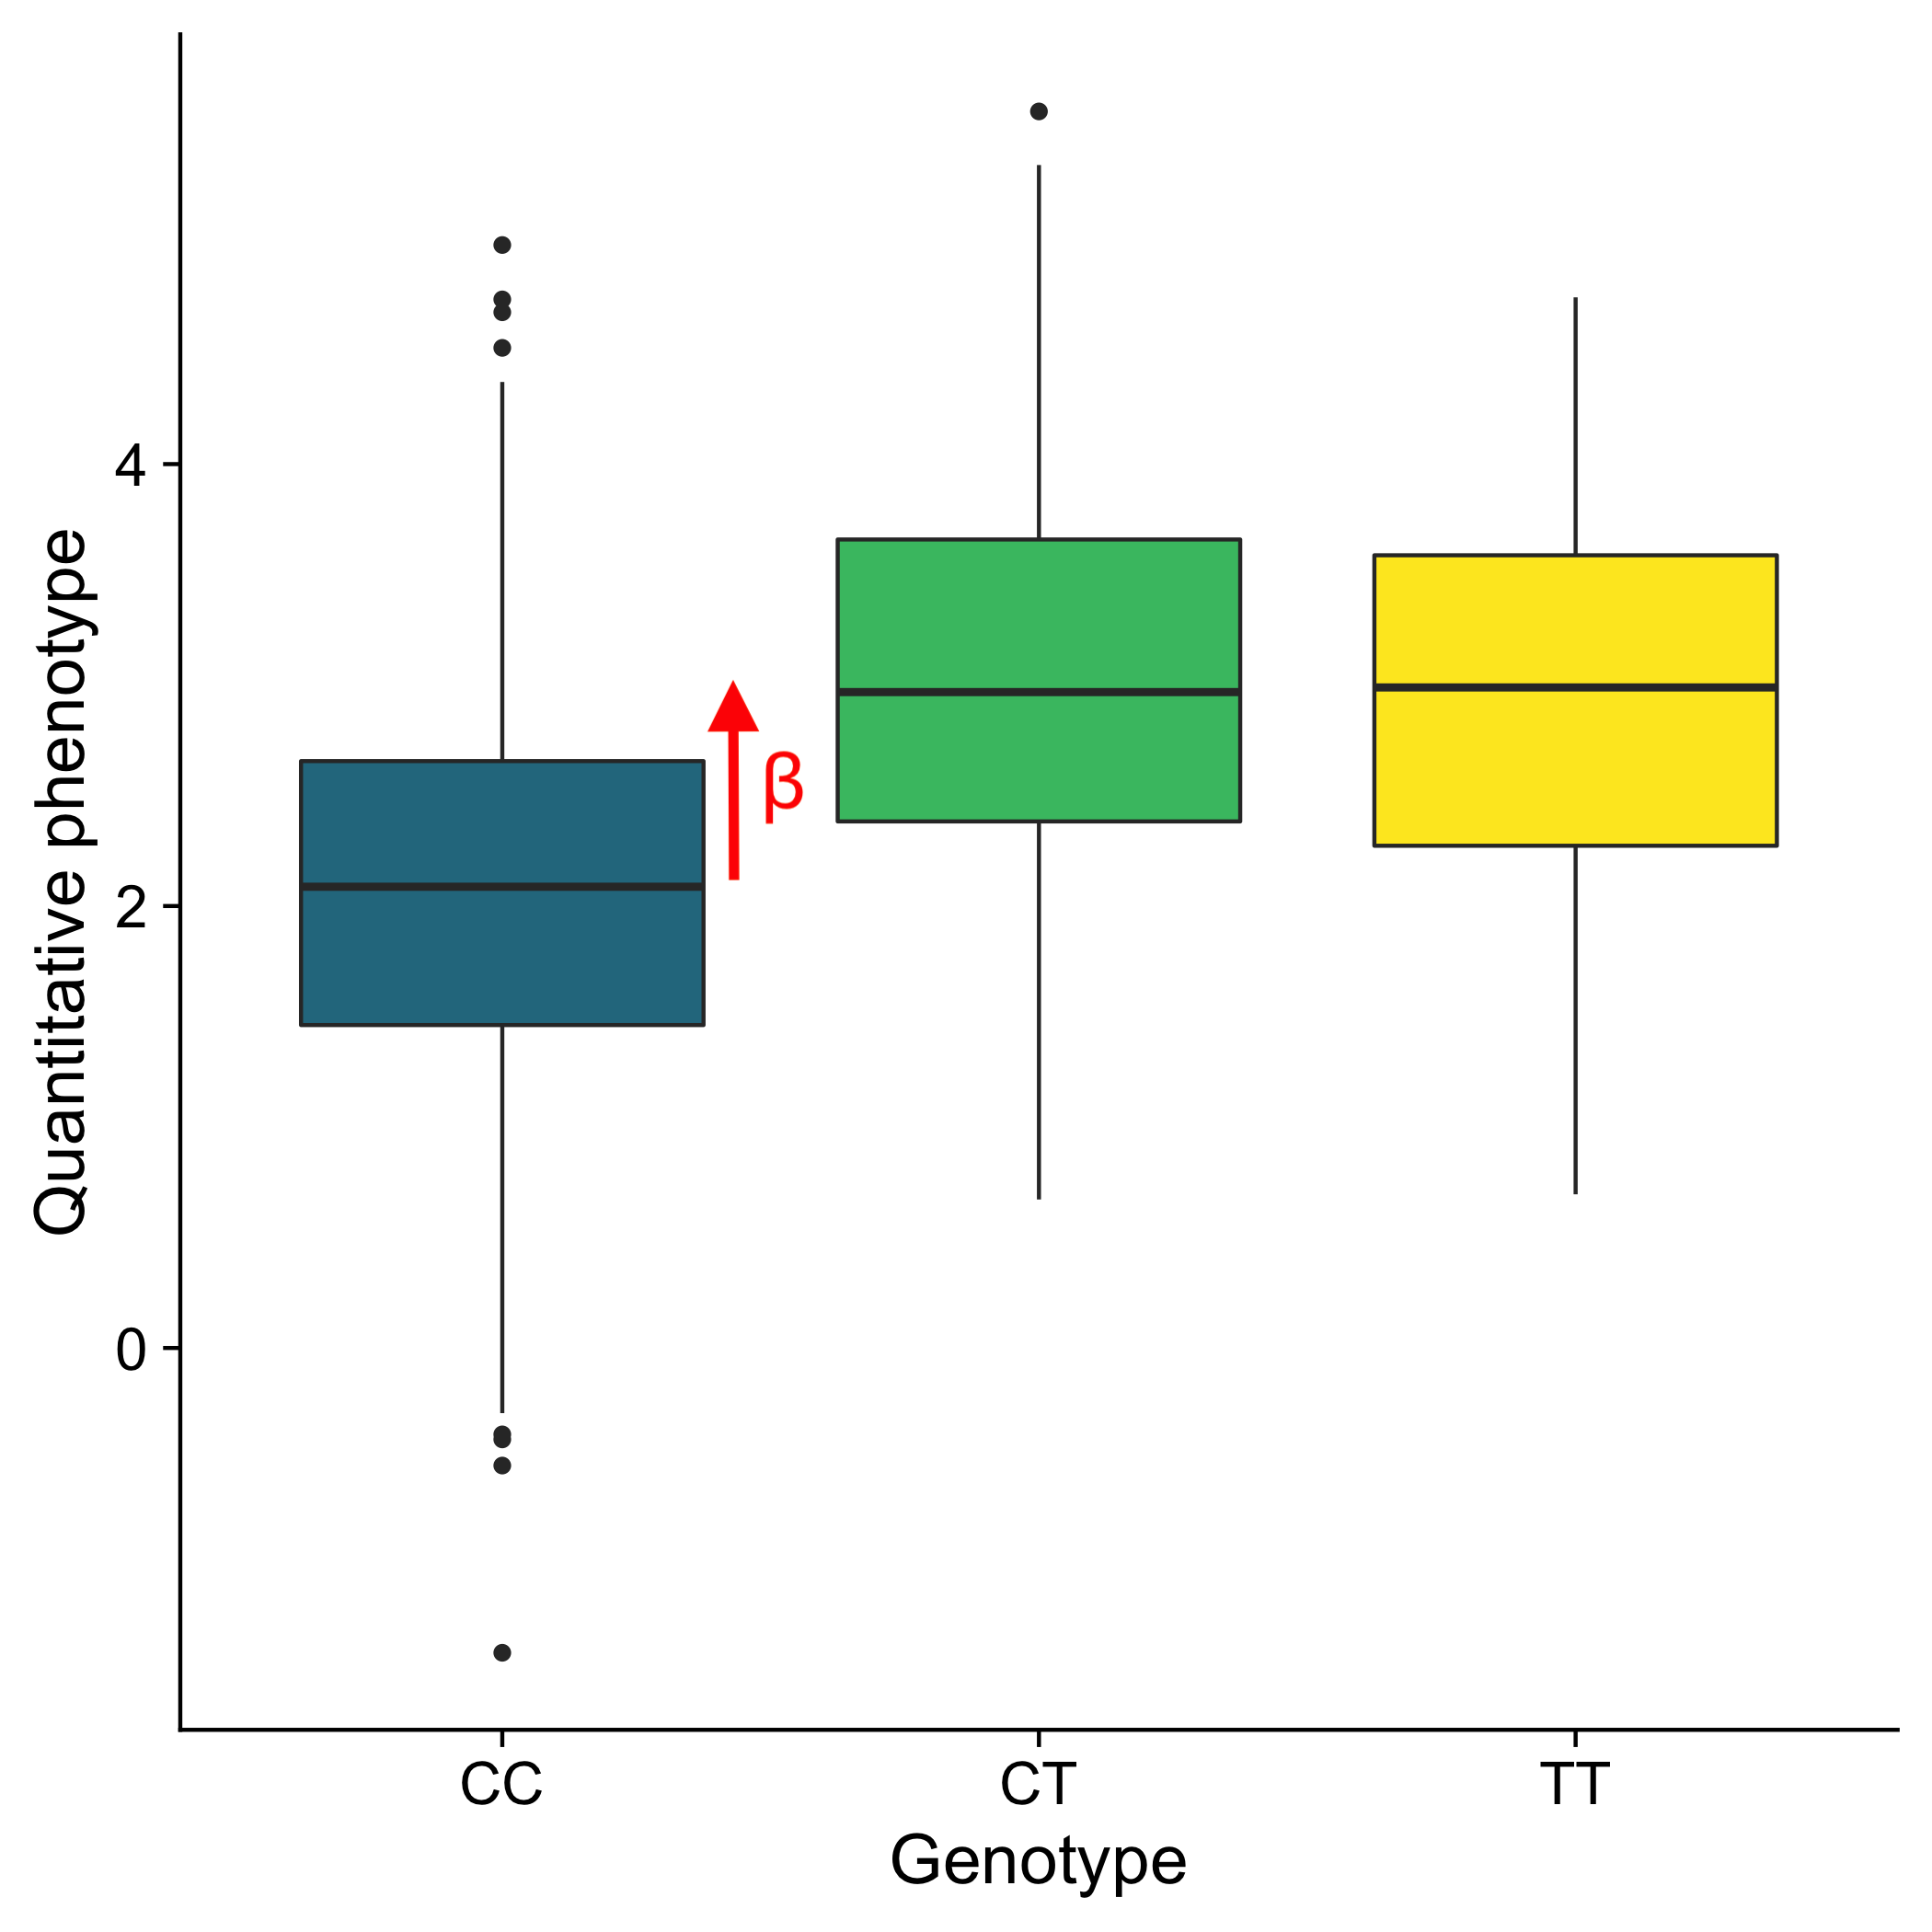
\includegraphics[scale=.08]{Figures/lm_dom.png}
	}
	
\end{frame}


\begin{frame}
	\frametitle{\bf Linear regression, with SNPs}
	or the `recessive model';
	\[
	y = \beta_0 + \beta\times I\{G== TT\}
	\]
	
	\centerline{
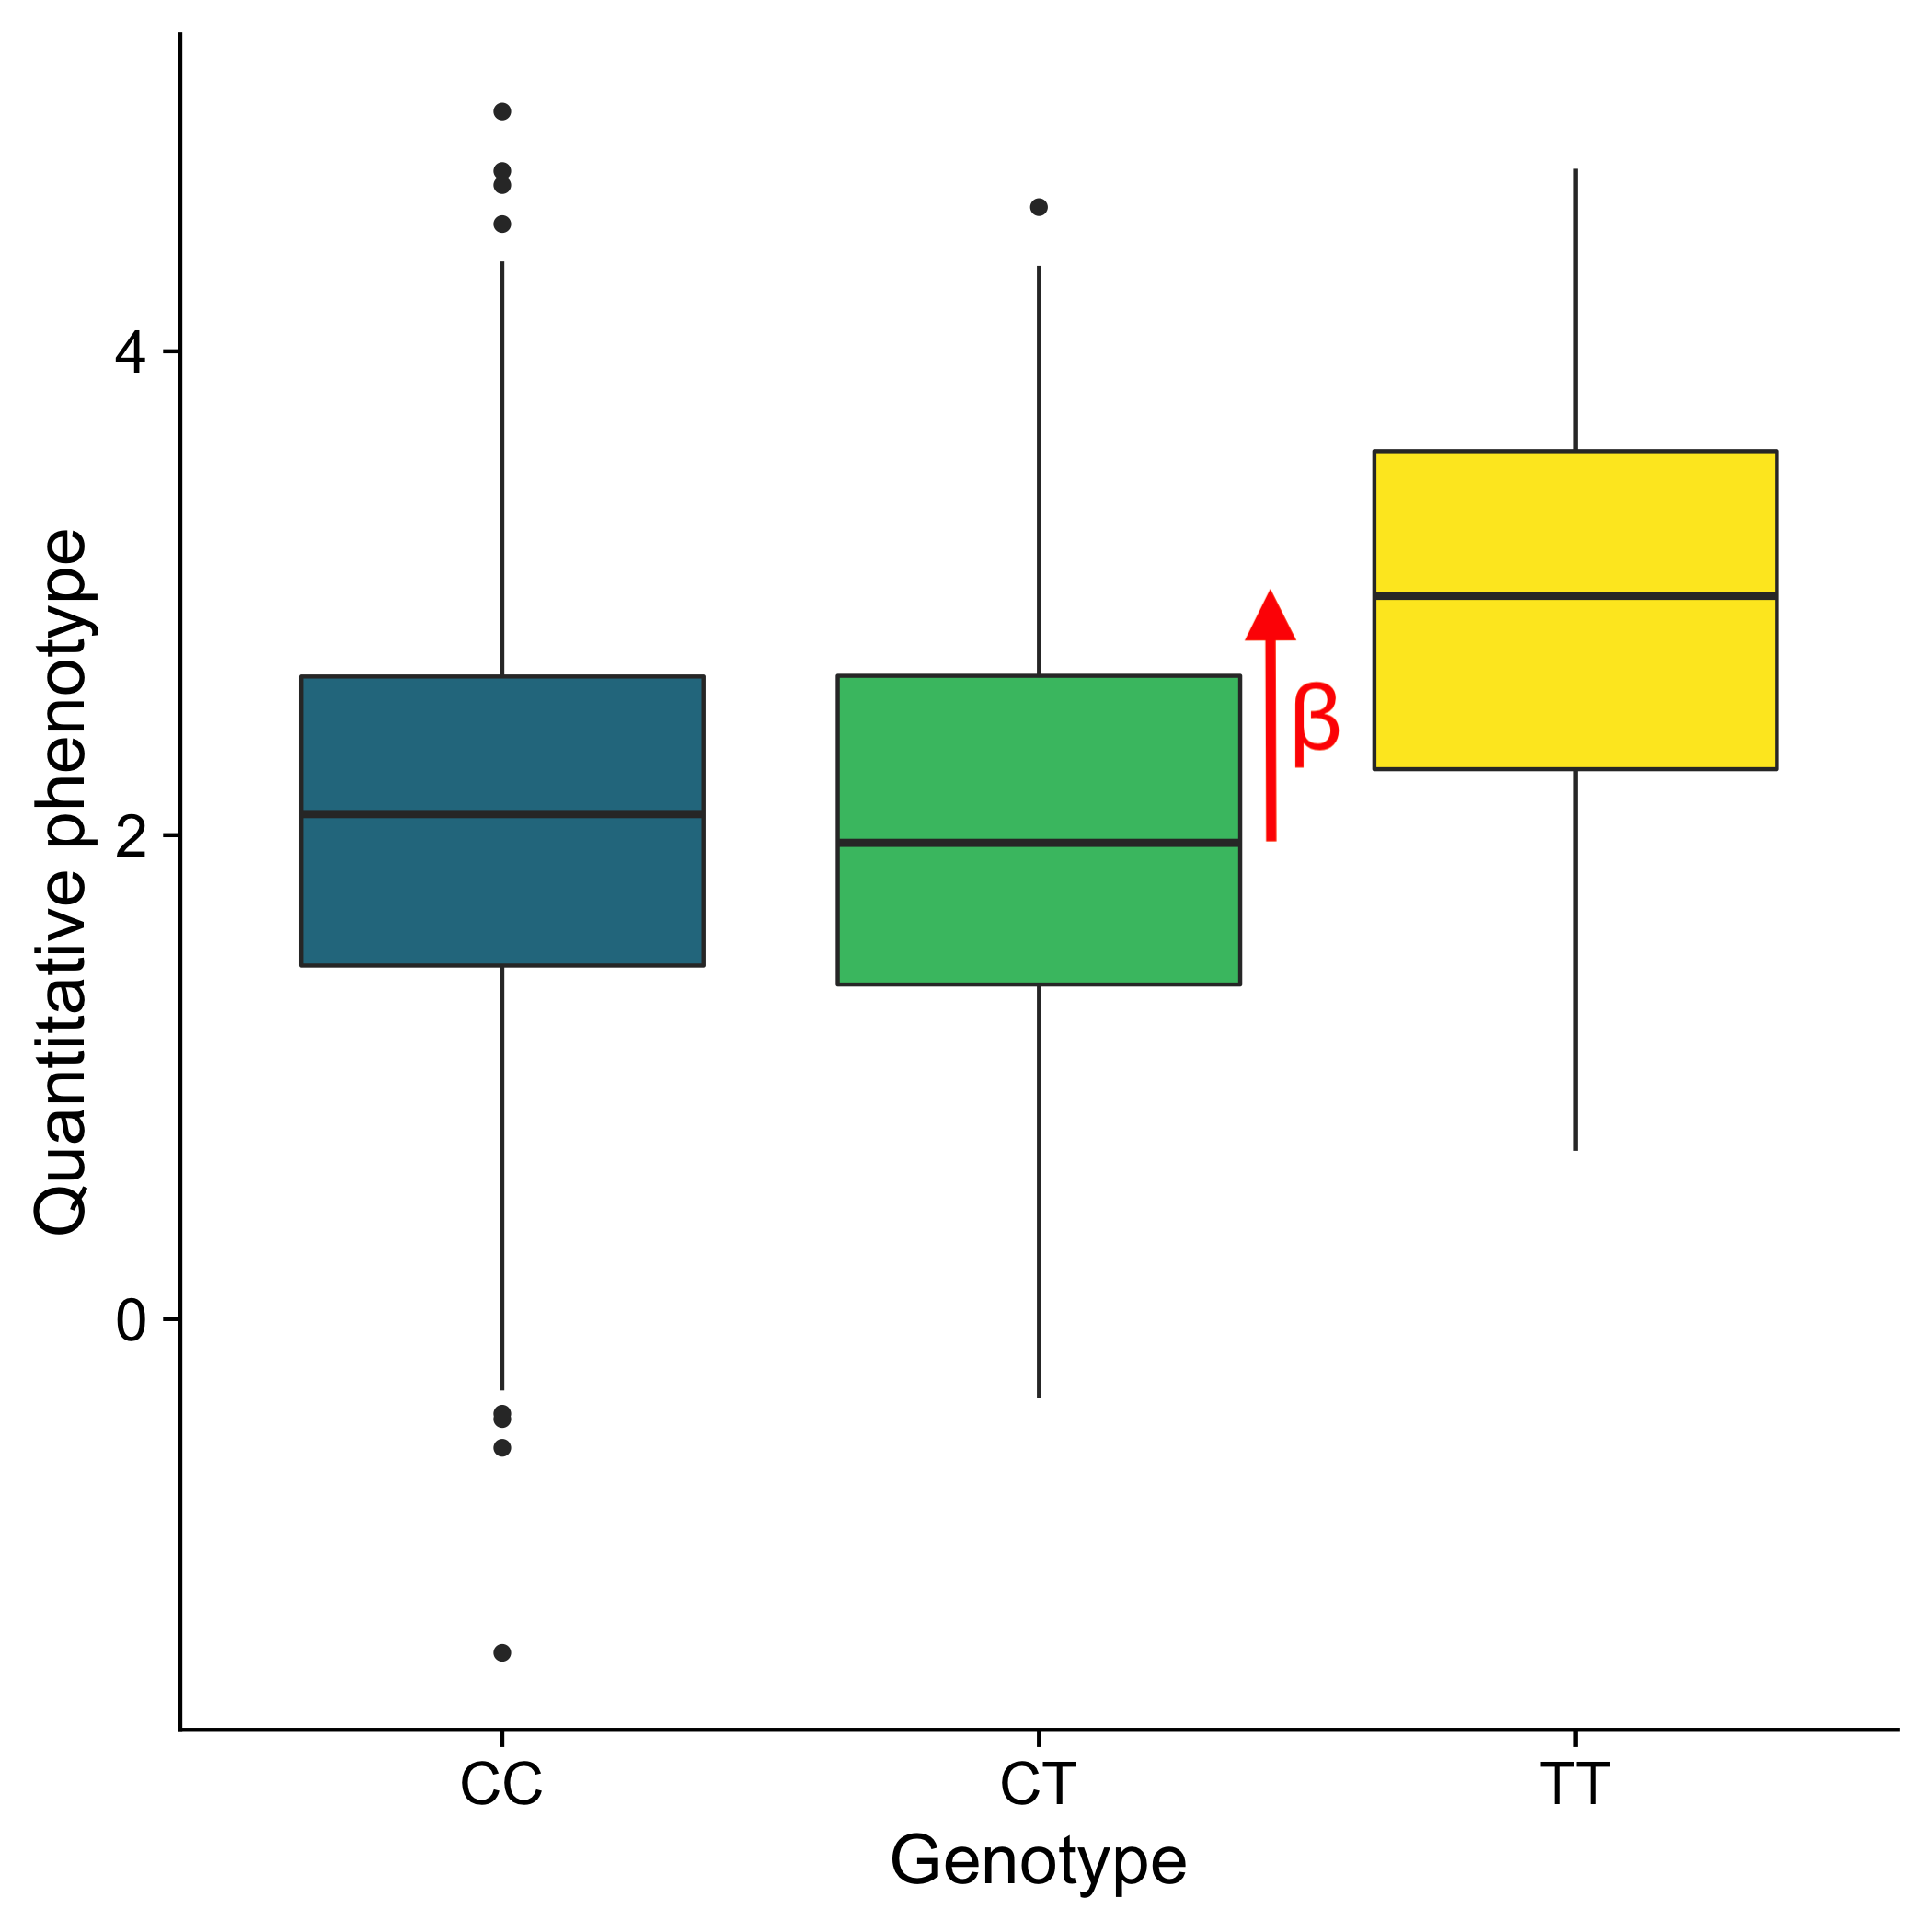
\includegraphics[scale=.08]{Figures/lm_rec.png}
	}
	
\end{frame}

\begin{frame}
	\frametitle{\bf Linear regression, with SNPs}
	Finally, the `two degrees of freedom model';
	\[
	y = \beta_0 + \beta_{CT}\times I\{G== CT\} + \beta_{TT}\times I\{G== TT\}
	\]
	
	\centerline{
	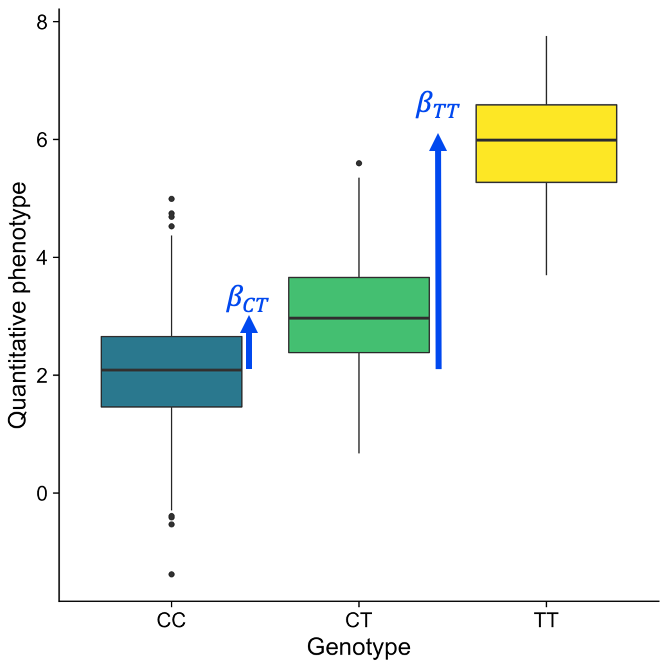
\includegraphics[scale=.3]{Figures/lm_cat.png}	}
	
\end{frame}


\begin{frame}
	\frametitle{\bf Additive Genetic Model}
	\begin{itemize}
				\item  Most GWAS perform single SNP association testing with linear regression assuming an additive model. 
		\item The coefficient of determination $(r^2)$ of an additive linear regression model  gives an estimate of the proportion of phenotypic variation that is explained by the SNP (or SNPs) in the model, e.g., the "SNP heritability" 
	\end{itemize}
\end{frame}


\begin{frame}
	\frametitle{\bf Additive Genetic Model}
	\begin{itemize}
		\item Consider the following additive model for  association testing with a quantitative trait and a SNP with alleles $C$ and $T$: 
		\[ Y=\beta_{0} + \beta_{1}G + \epsilon \]
		where $G$ is the number of copies of the allele $T$.
		\item What would your interpretation of $\epsilon$ be for this particular model?
	\end{itemize}
\end{frame}

\begin{frame}
	\frametitle{\bf Association Testing with Additive Model}
	\[ Y=\beta_{0} + \beta_{1}G + \epsilon \]
	\begin{itemize}
		\item Two test statistics for $H_0: \beta_{1}=0$ versus  $H_a: \beta_{1} \ne 0$ 
		\[T=\frac{\hat{\beta}_{1}}{\sqrt{var(\hat{\beta}_1)}} \sim \mathbf{t}_{N-2} \approx N(0,1) \mbox{ for large $N$}\]
		\[T^2=\frac{\hat{\beta}^2_{1}}{var(\hat{\beta}_1)} \sim \mathbf{F}_{1,N-2} \approx \chi^2_1\mbox{ for large $N$}\]
		where
		\[var(\hat{\beta}_1) =\frac{\sigma^2_{\epsilon}}{S_{GG}} \]
		and $S_{GG}$ is the corrected sum of squares for the $G_i$'s
	\end{itemize}
\end{frame}


\begin{frame}
	\frametitle{\bf Missing Heritability}	
	\vspace{-2em}
	\begin{figure}
		\centering
		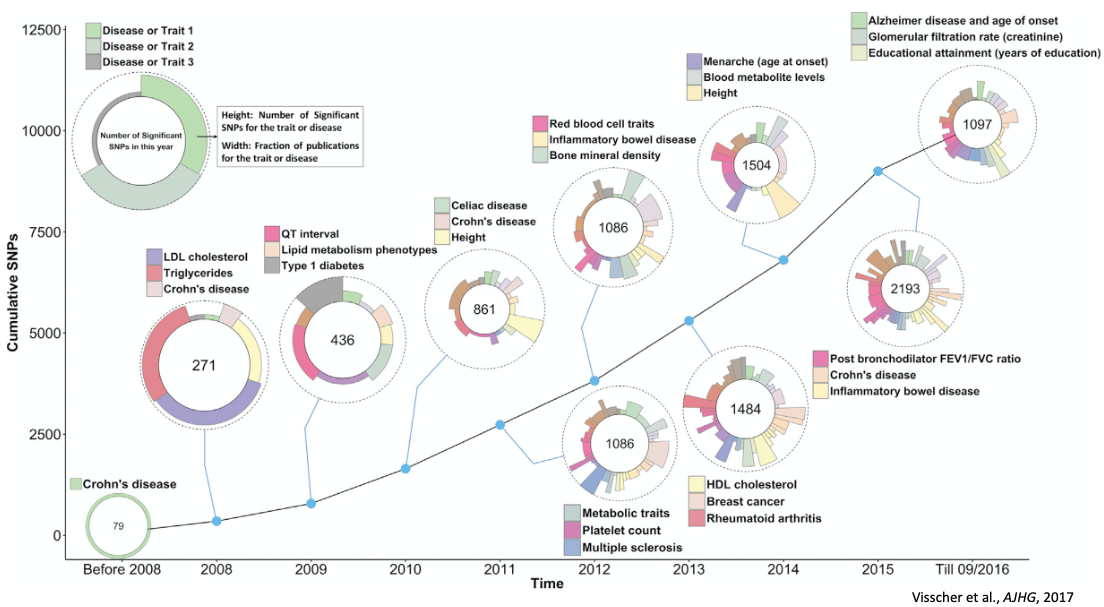
\includegraphics[scale=.25]{Figures/gwas_discoveries}
	\end{figure}
	\begin{itemize}
		\item Gap between SNP-based and pedigree-based heritability estimates
		\item Causal variants not well tagged? Rare variants involved?
	\end{itemize}
\end{frame}



\end{document}

